% Options for packages loaded elsewhere
\PassOptionsToPackage{unicode}{hyperref}
\PassOptionsToPackage{hyphens}{url}
%
\documentclass[
  ignorenonframetext,
]{beamer}
\usepackage{pgfpages}
\setbeamertemplate{caption}[numbered]
\setbeamertemplate{caption label separator}{: }
\setbeamercolor{caption name}{fg=normal text.fg}
\beamertemplatenavigationsymbolsempty
% Prevent slide breaks in the middle of a paragraph
\widowpenalties 1 10000
\raggedbottom
\setbeamertemplate{part page}{
  \centering
  \begin{beamercolorbox}[sep=16pt,center]{part title}
    \usebeamerfont{part title}\insertpart\par
  \end{beamercolorbox}
}
\setbeamertemplate{section page}{
  \centering
  \begin{beamercolorbox}[sep=12pt,center]{part title}
    \usebeamerfont{section title}\insertsection\par
  \end{beamercolorbox}
}
\setbeamertemplate{subsection page}{
  \centering
  \begin{beamercolorbox}[sep=8pt,center]{part title}
    \usebeamerfont{subsection title}\insertsubsection\par
  \end{beamercolorbox}
}
\AtBeginPart{
  \frame{\partpage}
}
\AtBeginSection{
  \ifbibliography
  \else
    \frame{\sectionpage}
  \fi
}
\AtBeginSubsection{
  \frame{\subsectionpage}
}
\usepackage{lmodern}
\usepackage{amssymb,amsmath}
\usepackage{ifxetex,ifluatex}
\ifnum 0\ifxetex 1\fi\ifluatex 1\fi=0 % if pdftex
  \usepackage[T1]{fontenc}
  \usepackage[utf8]{inputenc}
  \usepackage{textcomp} % provide euro and other symbols
\else % if luatex or xetex
  \usepackage{unicode-math}
  \defaultfontfeatures{Scale=MatchLowercase}
  \defaultfontfeatures[\rmfamily]{Ligatures=TeX,Scale=1}
\fi
\usetheme[]{Hannover}
\usecolortheme{dove}
\usefonttheme{structurebold}
% Use upquote if available, for straight quotes in verbatim environments
\IfFileExists{upquote.sty}{\usepackage{upquote}}{}
\IfFileExists{microtype.sty}{% use microtype if available
  \usepackage[]{microtype}
  \UseMicrotypeSet[protrusion]{basicmath} % disable protrusion for tt fonts
}{}
\makeatletter
\@ifundefined{KOMAClassName}{% if non-KOMA class
  \IfFileExists{parskip.sty}{%
    \usepackage{parskip}
  }{% else
    \setlength{\parindent}{0pt}
    \setlength{\parskip}{6pt plus 2pt minus 1pt}}
}{% if KOMA class
  \KOMAoptions{parskip=half}}
\makeatother
\usepackage{xcolor}
\IfFileExists{xurl.sty}{\usepackage{xurl}}{} % add URL line breaks if available
\IfFileExists{bookmark.sty}{\usepackage{bookmark}}{\usepackage{hyperref}}
\hypersetup{
  pdftitle={Session 3: What this lecture is about},
  pdfauthor={Levi Waldron},
  hidelinks,
  pdfcreator={LaTeX via pandoc}}
\urlstyle{same} % disable monospaced font for URLs
\newif\ifbibliography
\usepackage{color}
\usepackage{fancyvrb}
\newcommand{\VerbBar}{|}
\newcommand{\VERB}{\Verb[commandchars=\\\{\}]}
\DefineVerbatimEnvironment{Highlighting}{Verbatim}{commandchars=\\\{\}}
% Add ',fontsize=\small' for more characters per line
\usepackage{framed}
\definecolor{shadecolor}{RGB}{248,248,248}
\newenvironment{Shaded}{\begin{snugshade}}{\end{snugshade}}
\newcommand{\AlertTok}[1]{\textcolor[rgb]{0.94,0.16,0.16}{#1}}
\newcommand{\AnnotationTok}[1]{\textcolor[rgb]{0.56,0.35,0.01}{\textbf{\textit{#1}}}}
\newcommand{\AttributeTok}[1]{\textcolor[rgb]{0.77,0.63,0.00}{#1}}
\newcommand{\BaseNTok}[1]{\textcolor[rgb]{0.00,0.00,0.81}{#1}}
\newcommand{\BuiltInTok}[1]{#1}
\newcommand{\CharTok}[1]{\textcolor[rgb]{0.31,0.60,0.02}{#1}}
\newcommand{\CommentTok}[1]{\textcolor[rgb]{0.56,0.35,0.01}{\textit{#1}}}
\newcommand{\CommentVarTok}[1]{\textcolor[rgb]{0.56,0.35,0.01}{\textbf{\textit{#1}}}}
\newcommand{\ConstantTok}[1]{\textcolor[rgb]{0.00,0.00,0.00}{#1}}
\newcommand{\ControlFlowTok}[1]{\textcolor[rgb]{0.13,0.29,0.53}{\textbf{#1}}}
\newcommand{\DataTypeTok}[1]{\textcolor[rgb]{0.13,0.29,0.53}{#1}}
\newcommand{\DecValTok}[1]{\textcolor[rgb]{0.00,0.00,0.81}{#1}}
\newcommand{\DocumentationTok}[1]{\textcolor[rgb]{0.56,0.35,0.01}{\textbf{\textit{#1}}}}
\newcommand{\ErrorTok}[1]{\textcolor[rgb]{0.64,0.00,0.00}{\textbf{#1}}}
\newcommand{\ExtensionTok}[1]{#1}
\newcommand{\FloatTok}[1]{\textcolor[rgb]{0.00,0.00,0.81}{#1}}
\newcommand{\FunctionTok}[1]{\textcolor[rgb]{0.00,0.00,0.00}{#1}}
\newcommand{\ImportTok}[1]{#1}
\newcommand{\InformationTok}[1]{\textcolor[rgb]{0.56,0.35,0.01}{\textbf{\textit{#1}}}}
\newcommand{\KeywordTok}[1]{\textcolor[rgb]{0.13,0.29,0.53}{\textbf{#1}}}
\newcommand{\NormalTok}[1]{#1}
\newcommand{\OperatorTok}[1]{\textcolor[rgb]{0.81,0.36,0.00}{\textbf{#1}}}
\newcommand{\OtherTok}[1]{\textcolor[rgb]{0.56,0.35,0.01}{#1}}
\newcommand{\PreprocessorTok}[1]{\textcolor[rgb]{0.56,0.35,0.01}{\textit{#1}}}
\newcommand{\RegionMarkerTok}[1]{#1}
\newcommand{\SpecialCharTok}[1]{\textcolor[rgb]{0.00,0.00,0.00}{#1}}
\newcommand{\SpecialStringTok}[1]{\textcolor[rgb]{0.31,0.60,0.02}{#1}}
\newcommand{\StringTok}[1]{\textcolor[rgb]{0.31,0.60,0.02}{#1}}
\newcommand{\VariableTok}[1]{\textcolor[rgb]{0.00,0.00,0.00}{#1}}
\newcommand{\VerbatimStringTok}[1]{\textcolor[rgb]{0.31,0.60,0.02}{#1}}
\newcommand{\WarningTok}[1]{\textcolor[rgb]{0.56,0.35,0.01}{\textbf{\textit{#1}}}}
\usepackage{longtable,booktabs}
\usepackage{caption}
% Make caption package work with longtable
\makeatletter
\def\fnum@table{\tablename~\thetable}
\makeatother
\usepackage{graphicx,grffile}
\makeatletter
\def\maxwidth{\ifdim\Gin@nat@width>\linewidth\linewidth\else\Gin@nat@width\fi}
\def\maxheight{\ifdim\Gin@nat@height>\textheight\textheight\else\Gin@nat@height\fi}
\makeatother
% Scale images if necessary, so that they will not overflow the page
% margins by default, and it is still possible to overwrite the defaults
% using explicit options in \includegraphics[width, height, ...]{}
\setkeys{Gin}{width=\maxwidth,height=\maxheight,keepaspectratio}
% Set default figure placement to htbp
\makeatletter
\def\fps@figure{htbp}
\makeatother
\setlength{\emergencystretch}{3em} % prevent overfull lines
\providecommand{\tightlist}{%
  \setlength{\itemsep}{0pt}\setlength{\parskip}{0pt}}
\setcounter{secnumdepth}{-\maxdimen} % remove section numbering

\title{Session 3: What this lecture is about}
\author{Levi Waldron}
\date{}
\institute{CUNY SPH Biostatistics 2}

\begin{document}
\frame{\titlepage}

\hypertarget{learning-objectives-and-outline}{%
\section{Learning objectives and
outline}\label{learning-objectives-and-outline}}

\begin{frame}{Learning objectives}
\protect\hypertarget{learning-objectives}{}

\begin{enumerate}
\tightlist
\item
  Interpret main coefficients in logistic regression
\item
  Interpret interaction terms in logistic regression
\item
  Define and interpret model matrices for (generalized) linear models
\end{enumerate}

\end{frame}

\begin{frame}{Outline}
\protect\hypertarget{outline}{}

\begin{enumerate}
\tightlist
\item
  Review of GLM
\item
  Interpretation of logistic regression coefficients
\item
  Introduction to model matrices
\end{enumerate}

\end{frame}

\hypertarget{glm-review}{%
\section{GLM review}\label{glm-review}}

\begin{frame}{Components of GLM}
\protect\hypertarget{components-of-glm}{}

\begin{itemize}
\tightlist
\item
  \textbf{Random component} specifies the conditional distribution for
  the response variable

  \begin{itemize}
  \tightlist
  \item
    doesn't have to be normal
  \item
    can be any distribution in the ``exponential'' family of
    distributions
  \end{itemize}
\item
  \textbf{Systematic component} specifies linear function of predictors
  (linear predictor)
\item
  \textbf{Link} {[}denoted by g(.){]} specifies the relationship between
  the expected value of the random component and the systematic
  component

  \begin{itemize}
  \tightlist
  \item
    can be linear or nonlinear
  \end{itemize}
\end{itemize}

\end{frame}

\begin{frame}{Logistic Regression as GLM}
\protect\hypertarget{logistic-regression-as-glm}{}

\begin{itemize}
\item
  \textbf{The model}: \[
  Logit(P(x)) = log \left( \frac{P(x)}{1-P(x)} \right) = \beta_0 + \beta_1 x_{1i} + \beta_2 x_{2i} + ... + \beta_p x_{pi}
  \]
\item
  \textbf{Random component}: \(y_i\) follows a Binomial distribution
  (outcome is a binary variable)
\item
  \textbf{Systematic component}: linear predictor \[
  \beta_0 + \beta_1 x_{1i} + \beta_2 x_{2i} + ... + \beta_p x_{pi}
  \]
\item
  \textbf{Link function}: \emph{logit} (log of the odds that the event
  occurs)
\end{itemize}

\[
g(P(x)) = logit(P(x)) = log\left( \frac{P(x)}{1-P(x)} \right)
\]

\[
P(x) = g^{-1}\left( \beta_0 + \beta_1 x_{1i} + \beta_2 x_{2i} + ... + \beta_p x_{pi}
 \right)
\]

\end{frame}

\begin{frame}{Additive vs.~Multiplicative models}
\protect\hypertarget{additive-vs.-multiplicative-models}{}

\begin{itemize}
\tightlist
\item
  Linear regression is an \emph{additive} model

  \begin{itemize}
  \tightlist
  \item
    \emph{e.g.} for two binary variables \(\beta_1 = 1.5\),
    \(\beta_2 = 1.5\).
  \item
    If \(x_1=1\) and \(x_2=1\), this adds 3.0 to \(E(y|x)\)
  \end{itemize}
\item
  Logistic regression is a \emph{multiplicative} model

  \begin{itemize}
  \tightlist
  \item
    If \(x_1=1\) and \(x_2=1\), this adds 3.0 to \(log(\frac{P}{1-P})\)
  \item
    Odds-ratio \(\frac{P}{1-P}\) increases 20-fold: \(exp(1.5+1.5)\) or
    \(exp(1.5) * exp(1.5)\)
  \end{itemize}
\end{itemize}

\end{frame}

\begin{frame}[fragile]{Motivating example: contraceptive use data}
\protect\hypertarget{motivating-example-contraceptive-use-data}{}

From \url{http://data.princeton.edu/wws509/datasets/\#cuse}

\begin{verbatim}
##      age             education          wantsMore            notUsing     
##  Length:16          Length:16          Length:16          Min.   :  8.00  
##  Class :character   Class :character   Class :character   1st Qu.: 31.00  
##  Mode  :character   Mode  :character   Mode  :character   Median : 56.50  
##                                                           Mean   : 68.75  
##                                                           3rd Qu.: 85.75  
##                                                           Max.   :212.00  
##      using      
##  Min.   : 4.00  
##  1st Qu.: 9.50  
##  Median :29.00  
##  Mean   :31.69  
##  3rd Qu.:49.00  
##  Max.   :80.00
\end{verbatim}

\end{frame}

\begin{frame}[fragile]{Motivating example: contraceptive use data}
\protect\hypertarget{motivating-example-contraceptive-use-data-1}{}

Univariate regression to ``wants more children'' only:

\tiny

\begin{Shaded}
\begin{Highlighting}[]
\NormalTok{fit <-}\StringTok{ }\KeywordTok{glm}\NormalTok{(}\KeywordTok{cbind}\NormalTok{(using, notUsing) }\OperatorTok{~}\StringTok{ }\NormalTok{wantsMore, }
           \DataTypeTok{data=}\NormalTok{cuse, }\DataTypeTok{family=}\KeywordTok{binomial}\NormalTok{(}\StringTok{"logit"}\NormalTok{))}
\end{Highlighting}
\end{Shaded}

Estimate

Std. Error

z value

Pr(\textgreater\textbar z\textbar)

(Intercept)

-0.1864

0.0797

-2.34

0.0194

wantsMoreyes

-1.0486

0.1107

-9.48

0.0000

\begin{itemize}
\tightlist
\item
  Interpretation of this table:

  \begin{itemize}
  \tightlist
  \item
    Coefficients for \textbf{(Intercept)} and \textbf{dummy variables}
  \item
    Coefficients are normally distributed when assumptions are correct
  \end{itemize}
\end{itemize}

\end{frame}

\begin{frame}{Interpretation of coefficients}
\protect\hypertarget{interpretation-of-coefficients}{}

\begin{figure}
\centering
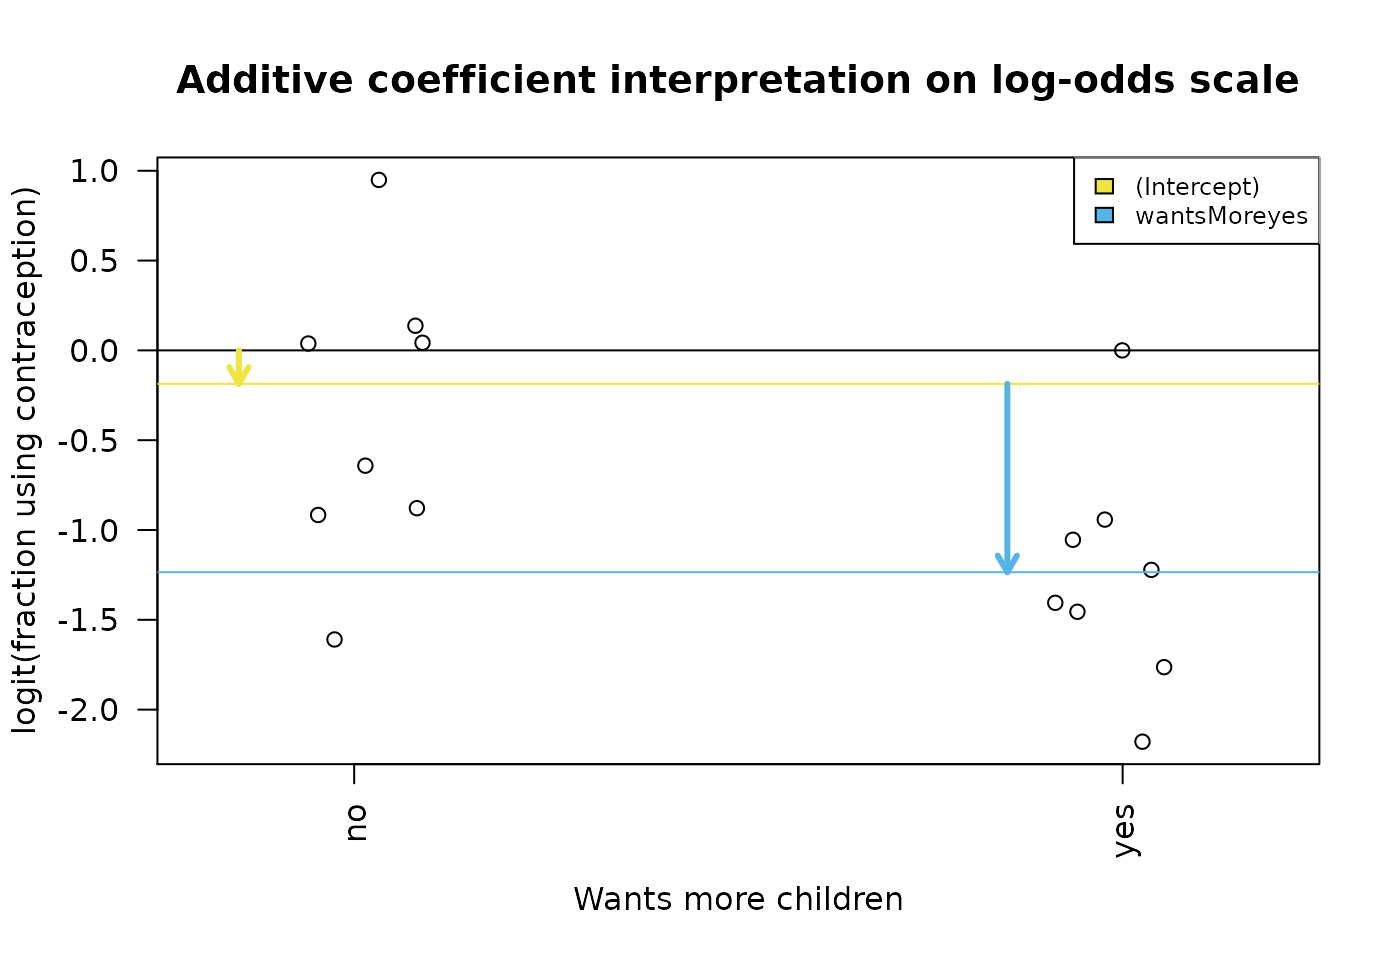
\includegraphics{../docs/articles/session_lecture_files/figure-beamer/main_coef-1.pdf}
\caption{Diagram of the estimated coefficients in the GLM. The green
arrow indicates the Intercept term, which goes from zero to the mean of
the reference group (here the `wantsMore = no' samples). The orange
arrow indicates the difference in log-odds of the yes group minus the no
group, which is negative in this example. The circles show the
individual samples, jittered horizontally to avoid overplotting.}
\end{figure}

\end{frame}

\begin{frame}[fragile]{Regression on \textbf{age}}
\protect\hypertarget{regression-on-age}{}

There are four age groups:

\begin{Shaded}
\begin{Highlighting}[]
\NormalTok{fit <-}\StringTok{ }\KeywordTok{glm}\NormalTok{(}\KeywordTok{cbind}\NormalTok{(using, notUsing) }\OperatorTok{~}\StringTok{ }\NormalTok{age, }
           \DataTypeTok{data=}\NormalTok{cuse, }\DataTypeTok{family=}\KeywordTok{binomial}\NormalTok{(}\StringTok{"logit"}\NormalTok{))}
\end{Highlighting}
\end{Shaded}

Estimate

Std. Error

z value

Pr(\textgreater\textbar z\textbar)

(Intercept)

-1.5072

0.1303

-11.57

0.0000

age25-29

0.4607

0.1727

2.67

0.0077

age30-39

1.0483

0.1544

6.79

0.0000

age40-49

1.4246

0.1940

7.35

0.0000

\begin{itemize}
\tightlist
\item
  Interpretation of the dummy variables \texttt{age25-29},
  \texttt{age30-39}, \texttt{age40-49}
\end{itemize}

\end{frame}

\begin{frame}{Regression with multiple predictors - model formulae:}
\protect\hypertarget{regression-with-multiple-predictors---model-formulae}{}

\begin{longtable}[]{@{}lll@{}}
\toprule
\begin{minipage}[b]{0.14\columnwidth}\raggedright
symbol\strut
\end{minipage} & \begin{minipage}[b]{0.24\columnwidth}\raggedright
example\strut
\end{minipage} & \begin{minipage}[b]{0.53\columnwidth}\raggedright
meaning\strut
\end{minipage}\tabularnewline
\midrule
\endhead
\begin{minipage}[t]{0.14\columnwidth}\raggedright
+\strut
\end{minipage} & \begin{minipage}[t]{0.24\columnwidth}\raggedright
+ x\strut
\end{minipage} & \begin{minipage}[t]{0.53\columnwidth}\raggedright
include this variable\strut
\end{minipage}\tabularnewline
\begin{minipage}[t]{0.14\columnwidth}\raggedright
-\strut
\end{minipage} & \begin{minipage}[t]{0.24\columnwidth}\raggedright
- x\strut
\end{minipage} & \begin{minipage}[t]{0.53\columnwidth}\raggedright
delete this variable\strut
\end{minipage}\tabularnewline
\begin{minipage}[t]{0.14\columnwidth}\raggedright
:\strut
\end{minipage} & \begin{minipage}[t]{0.24\columnwidth}\raggedright
x : z\strut
\end{minipage} & \begin{minipage}[t]{0.53\columnwidth}\raggedright
include the interaction\strut
\end{minipage}\tabularnewline
\begin{minipage}[t]{0.14\columnwidth}\raggedright
*\strut
\end{minipage} & \begin{minipage}[t]{0.24\columnwidth}\raggedright
x * z\strut
\end{minipage} & \begin{minipage}[t]{0.53\columnwidth}\raggedright
include these variables and their interactions\strut
\end{minipage}\tabularnewline
\begin{minipage}[t]{0.14\columnwidth}\raggedright
\^{}\strut
\end{minipage} & \begin{minipage}[t]{0.24\columnwidth}\raggedright
(u + v + w)\^{}3\strut
\end{minipage} & \begin{minipage}[t]{0.53\columnwidth}\raggedright
include these variables and all interactions up to three way\strut
\end{minipage}\tabularnewline
\begin{minipage}[t]{0.14\columnwidth}\raggedright
1\strut
\end{minipage} & \begin{minipage}[t]{0.24\columnwidth}\raggedright
-1\strut
\end{minipage} & \begin{minipage}[t]{0.53\columnwidth}\raggedright
intercept: delete the intercept\strut
\end{minipage}\tabularnewline
\bottomrule
\end{longtable}

\end{frame}

\begin{frame}[fragile]{Regression on \textbf{age} and
\textbf{wantsMore}}
\protect\hypertarget{regression-on-age-and-wantsmore}{}

\begin{Shaded}
\begin{Highlighting}[]
\NormalTok{fit <-}\StringTok{ }\KeywordTok{glm}\NormalTok{(}\KeywordTok{cbind}\NormalTok{(using, notUsing) }\OperatorTok{~}\StringTok{ }\NormalTok{age }\OperatorTok{+}\StringTok{ }\NormalTok{wantsMore, }
           \DataTypeTok{data=}\NormalTok{cuse, }\DataTypeTok{family=}\KeywordTok{binomial}\NormalTok{(}\StringTok{"logit"}\NormalTok{))}
\end{Highlighting}
\end{Shaded}

Estimate

Std. Error

z value

Pr(\textgreater\textbar z\textbar)

(Intercept)

-0.8698

0.1571

-5.54

0.0000

age25-29

0.3678

0.1754

2.10

0.0360

age30-39

0.8078

0.1598

5.06

0.0000

age40-49

1.0226

0.2039

5.01

0.0000

wantsMoreyes

-0.8241

0.1171

-7.04

0.0000

\end{frame}

\begin{frame}{Interaction / Effect Modification}
\protect\hypertarget{interaction-effect-modification}{}

\begin{itemize}
\tightlist
\item
  What if we want to know whether the effect of age is modified by
  whether the woman wants more children or not?
\end{itemize}

Interaction is modeled as the product of two covariates: \[
E[y|x] = \beta_0 + \beta_1 x_1 + \beta_2 x_2 + \beta_{12} x_1*x_2
\]

\end{frame}

\begin{frame}[fragile]{Interaction / Effect Modification (cont'd)}
\protect\hypertarget{interaction-effect-modification-contd}{}

\begin{Shaded}
\begin{Highlighting}[]
\NormalTok{fit <-}\StringTok{ }\KeywordTok{glm}\NormalTok{(}\KeywordTok{cbind}\NormalTok{(using, notUsing) }\OperatorTok{~}\StringTok{ }\NormalTok{age }\OperatorTok{*}\StringTok{ }\NormalTok{wantsMore, }
           \DataTypeTok{data=}\NormalTok{cuse, }\DataTypeTok{family=}\KeywordTok{binomial}\NormalTok{(}\StringTok{"logit"}\NormalTok{))}
\end{Highlighting}
\end{Shaded}

Estimate

Std. Error

z value

Pr(\textgreater\textbar z\textbar)

(Intercept)

-1.4553

0.2968

-4.90

0.0000

age25-29

0.6354

0.3564

1.78

0.0746

age30-39

1.5411

0.3183

4.84

0.0000

age40-49

1.7643

0.3435

5.14

0.0000

wantsMoreyes

-0.0640

0.3303

-0.19

0.8464

age25-29:wantsMoreyes

-0.2672

0.4091

-0.65

0.5137

age30-39:wantsMoreyes

-1.0905

0.3733

-2.92

0.0035

age40-49:wantsMoreyes

-1.3671

0.4834

-2.83

0.0047

\end{frame}

\hypertarget{the-design-matrix}{%
\section{The Design Matrix}\label{the-design-matrix}}

\begin{frame}{What is the design matrix, and why?}
\protect\hypertarget{what-is-the-design-matrix-and-why}{}

\begin{itemize}
\tightlist
\item
  \textbf{What?} The design matrix is the most generic, flexible way to
  specify them
\item
  \textbf{Why?} There are multiple possible and reasonable regression
  models for a given study design.
\end{itemize}

\end{frame}

\begin{frame}{Matrix notation for the multiple linear regression model}
\protect\hypertarget{matrix-notation-for-the-multiple-linear-regression-model}{}

\[
\,
\begin{pmatrix}
Y_1\\
Y_2\\
\vdots\\
Y_N
\end{pmatrix} = 
\begin{pmatrix}
1&x_1\\
1&x_2\\
\vdots\\
1&x_N
\end{pmatrix}
\begin{pmatrix}
\beta_0\\
\beta_1
\end{pmatrix} +
\begin{pmatrix}
\varepsilon_1\\
\varepsilon_2\\
\vdots\\
\varepsilon_N
\end{pmatrix}
\]

or simply:

\[
\mathbf{Y}=\mathbf{X}\boldsymbol{\beta}+\boldsymbol{\varepsilon}
\]

\begin{itemize}
\tightlist
\item
  The design matrix is \(\mathbf{X}\)

  \begin{itemize}
  \tightlist
  \item
    which the computer will take as a given when solving for
    \(\boldsymbol{\beta}\) by minimizing the sum of squares of residuals
    \(\boldsymbol{\varepsilon}\), or maximizing likelihood.
  \end{itemize}
\end{itemize}

\end{frame}

\begin{frame}[fragile]{Choice of design matrix}
\protect\hypertarget{choice-of-design-matrix}{}

\begin{itemize}
\tightlist
\item
  The model formula encodes a default model matrix, e.g.:
\end{itemize}

\begin{Shaded}
\begin{Highlighting}[]
\NormalTok{group <-}\StringTok{ }\KeywordTok{factor}\NormalTok{( }\KeywordTok{c}\NormalTok{(}\DecValTok{1}\NormalTok{, }\DecValTok{1}\NormalTok{, }\DecValTok{2}\NormalTok{, }\DecValTok{2}\NormalTok{) )}
\KeywordTok{model.matrix}\NormalTok{(}\OperatorTok{~}\StringTok{ }\NormalTok{group)}
\end{Highlighting}
\end{Shaded}

\begin{verbatim}
##   (Intercept) group2
## 1           1      0
## 2           1      0
## 3           1      1
## 4           1      1
## attr(,"assign")
## [1] 0 1
## attr(,"contrasts")
## attr(,"contrasts")$group
## [1] "contr.treatment"
\end{verbatim}

\end{frame}

\begin{frame}[fragile]{Choice of design matrix (cont'd)}
\protect\hypertarget{choice-of-design-matrix-contd}{}

What if we forgot to code group as a factor?

\begin{Shaded}
\begin{Highlighting}[]
\NormalTok{group <-}\StringTok{ }\KeywordTok{c}\NormalTok{(}\DecValTok{1}\NormalTok{, }\DecValTok{1}\NormalTok{, }\DecValTok{2}\NormalTok{, }\DecValTok{2}\NormalTok{)}
\KeywordTok{model.matrix}\NormalTok{(}\OperatorTok{~}\StringTok{ }\NormalTok{group)}
\end{Highlighting}
\end{Shaded}

\begin{verbatim}
##   (Intercept) group
## 1           1     1
## 2           1     1
## 3           1     2
## 4           1     2
## attr(,"assign")
## [1] 0 1
\end{verbatim}

\end{frame}

\begin{frame}[fragile]{More groups, still one variable}
\protect\hypertarget{more-groups-still-one-variable}{}

\begin{Shaded}
\begin{Highlighting}[]
\NormalTok{group <-}\StringTok{ }\KeywordTok{factor}\NormalTok{(}\KeywordTok{c}\NormalTok{(}\DecValTok{1}\NormalTok{,}\DecValTok{1}\NormalTok{,}\DecValTok{2}\NormalTok{,}\DecValTok{2}\NormalTok{,}\DecValTok{3}\NormalTok{,}\DecValTok{3}\NormalTok{))}
\KeywordTok{model.matrix}\NormalTok{(}\OperatorTok{~}\StringTok{ }\NormalTok{group)}
\end{Highlighting}
\end{Shaded}

\begin{verbatim}
##   (Intercept) group2 group3
## 1           1      0      0
## 2           1      0      0
## 3           1      1      0
## 4           1      1      0
## 5           1      0      1
## 6           1      0      1
## attr(,"assign")
## [1] 0 1 1
## attr(,"contrasts")
## attr(,"contrasts")$group
## [1] "contr.treatment"
\end{verbatim}

\end{frame}

\begin{frame}[fragile]{Changing the baseline group}
\protect\hypertarget{changing-the-baseline-group}{}

\begin{Shaded}
\begin{Highlighting}[]
\NormalTok{group <-}\StringTok{ }\KeywordTok{factor}\NormalTok{(}\KeywordTok{c}\NormalTok{(}\DecValTok{1}\NormalTok{,}\DecValTok{1}\NormalTok{,}\DecValTok{2}\NormalTok{,}\DecValTok{2}\NormalTok{,}\DecValTok{3}\NormalTok{,}\DecValTok{3}\NormalTok{))}
\NormalTok{group <-}\StringTok{ }\KeywordTok{relevel}\NormalTok{(}\DataTypeTok{x=}\NormalTok{group, }\DataTypeTok{ref=}\DecValTok{3}\NormalTok{)}
\KeywordTok{model.matrix}\NormalTok{(}\OperatorTok{~}\StringTok{ }\NormalTok{group)}
\end{Highlighting}
\end{Shaded}

\begin{verbatim}
##   (Intercept) group1 group2
## 1           1      1      0
## 2           1      1      0
## 3           1      0      1
## 4           1      0      1
## 5           1      0      0
## 6           1      0      0
## attr(,"assign")
## [1] 0 1 1
## attr(,"contrasts")
## attr(,"contrasts")$group
## [1] "contr.treatment"
\end{verbatim}

\end{frame}

\begin{frame}[fragile]{More than one variable}
\protect\hypertarget{more-than-one-variable}{}

\begin{Shaded}
\begin{Highlighting}[]
\NormalTok{agegroup <-}\StringTok{ }\KeywordTok{factor}\NormalTok{(}\KeywordTok{c}\NormalTok{(}\DecValTok{1}\NormalTok{,}\DecValTok{1}\NormalTok{,}\DecValTok{1}\NormalTok{,}\DecValTok{1}\NormalTok{,}\DecValTok{2}\NormalTok{,}\DecValTok{2}\NormalTok{,}\DecValTok{2}\NormalTok{,}\DecValTok{2}\NormalTok{))}
\NormalTok{wantsMore <-}\StringTok{ }\KeywordTok{factor}\NormalTok{(}\KeywordTok{c}\NormalTok{(}\StringTok{"y"}\NormalTok{,}\StringTok{"y"}\NormalTok{,}\StringTok{"n"}\NormalTok{,}\StringTok{"n"}\NormalTok{,}\StringTok{"y"}\NormalTok{,}\StringTok{"y"}\NormalTok{,}\StringTok{"n"}\NormalTok{,}\StringTok{"n"}\NormalTok{))}
\KeywordTok{model.matrix}\NormalTok{(}\OperatorTok{~}\StringTok{ }\NormalTok{agegroup }\OperatorTok{+}\StringTok{ }\NormalTok{wantsMore)}
\end{Highlighting}
\end{Shaded}

\begin{verbatim}
##   (Intercept) agegroup2 wantsMorey
## 1           1         0          1
## 2           1         0          1
## 3           1         0          0
## 4           1         0          0
## 5           1         1          1
## 6           1         1          1
## 7           1         1          0
## 8           1         1          0
## attr(,"assign")
## [1] 0 1 2
## attr(,"contrasts")
## attr(,"contrasts")$agegroup
## [1] "contr.treatment"
## 
## attr(,"contrasts")$wantsMore
## [1] "contr.treatment"
\end{verbatim}

\end{frame}

\begin{frame}[fragile]{With an interaction term}
\protect\hypertarget{with-an-interaction-term}{}

\begin{Shaded}
\begin{Highlighting}[]
\KeywordTok{model.matrix}\NormalTok{(}\OperatorTok{~}\StringTok{ }\NormalTok{agegroup }\OperatorTok{+}\StringTok{ }\NormalTok{wantsMore }\OperatorTok{+}\StringTok{ }\NormalTok{agegroup}\OperatorTok{:}\NormalTok{wantsMore)}
\end{Highlighting}
\end{Shaded}

\begin{verbatim}
##   (Intercept) agegroup2 wantsMorey agegroup2:wantsMorey
## 1           1         0          1                    0
## 2           1         0          1                    0
## 3           1         0          0                    0
## 4           1         0          0                    0
## 5           1         1          1                    1
## 6           1         1          1                    1
## 7           1         1          0                    0
## 8           1         1          0                    0
## attr(,"assign")
## [1] 0 1 2 3
## attr(,"contrasts")
## attr(,"contrasts")$agegroup
## [1] "contr.treatment"
## 
## attr(,"contrasts")$wantsMore
## [1] "contr.treatment"
\end{verbatim}

\end{frame}

\begin{frame}[fragile]{Design matrix to contrast what we want}
\protect\hypertarget{design-matrix-to-contrast-what-we-want}{}

\begin{itemize}
\tightlist
\item
  Contraceptive use example

  \begin{itemize}
  \tightlist
  \item
    Is the effect of wanting more children different for 40-49 year-olds
    than for \textless25 year-olds is answered by the term
    \texttt{age40-49:wantsMoreyes} in a model with interaction terms:
  \end{itemize}
\end{itemize}

\begin{Shaded}
\begin{Highlighting}[]
\NormalTok{fitX <-}\StringTok{ }\KeywordTok{glm}\NormalTok{(}\KeywordTok{cbind}\NormalTok{(using, notUsing) }\OperatorTok{~}\StringTok{ }\NormalTok{age }\OperatorTok{*}\StringTok{ }\NormalTok{wantsMore, }
           \DataTypeTok{data=}\NormalTok{cuse, }\DataTypeTok{family=}\KeywordTok{binomial}\NormalTok{(}\StringTok{"logit"}\NormalTok{))}
\KeywordTok{summary}\NormalTok{(fitX)}
\end{Highlighting}
\end{Shaded}

\begin{verbatim}
## 
## Call:
## glm(formula = cbind(using, notUsing) ~ age * wantsMore, family = binomial("logit"), 
##     data = cuse)
## 
## Deviance Residuals: 
##      Min        1Q    Median        3Q       Max  
## -1.67001  -0.85288   0.02621   0.72300   2.18925  
## 
## Coefficients:
##                       Estimate Std. Error z value Pr(>|z|)    
## (Intercept)            -1.4553     0.2968  -4.903 9.43e-07 ***
## age25-29                0.6354     0.3564   1.783  0.07463 .  
## age30-39                1.5412     0.3183   4.842 1.29e-06 ***
## age40-49                1.7643     0.3435   5.136 2.80e-07 ***
## wantsMoreyes           -0.0640     0.3303  -0.194  0.84637    
## age25-29:wantsMoreyes  -0.2672     0.4091  -0.653  0.51366    
## age30-39:wantsMoreyes  -1.0905     0.3733  -2.921  0.00349 ** 
## age40-49:wantsMoreyes  -1.3672     0.4834  -2.828  0.00468 ** 
## ---
## Signif. codes:  0 '***' 0.001 '**' 0.01 '*' 0.05 '.' 0.1 ' ' 1
## 
## (Dispersion parameter for binomial family taken to be 1)
## 
##     Null deviance: 165.772  on 15  degrees of freedom
## Residual deviance:  20.099  on  8  degrees of freedom
## AIC: 107.61
## 
## Number of Fisher Scoring iterations: 4
\end{verbatim}

\end{frame}

\begin{frame}[fragile]{Design matrix to contrast what we want (cont'd)}
\protect\hypertarget{design-matrix-to-contrast-what-we-want-contd}{}

\begin{itemize}
\tightlist
\item
  What if we want to ask this question for 40-49 year-olds vs.~30-39
  year-olds?
\end{itemize}

The desired contrast is:

\texttt{age40-49:wantsMoreyes\ -\ age30-39:wantsMoreyes}

There are many ways to construct this design, one is with
\texttt{library(multcomp)}:

\begin{Shaded}
\begin{Highlighting}[]
\KeywordTok{names}\NormalTok{(}\KeywordTok{coef}\NormalTok{(fitX))}
\end{Highlighting}
\end{Shaded}

\begin{verbatim}
## [1] "(Intercept)"           "age25-29"              "age30-39"             
## [4] "age40-49"              "wantsMoreyes"          "age25-29:wantsMoreyes"
## [7] "age30-39:wantsMoreyes" "age40-49:wantsMoreyes"
\end{verbatim}

\begin{Shaded}
\begin{Highlighting}[]
\NormalTok{contmat <-}\StringTok{ }\KeywordTok{matrix}\NormalTok{(}\KeywordTok{c}\NormalTok{(}\DecValTok{0}\NormalTok{,}\DecValTok{0}\NormalTok{,}\DecValTok{0}\NormalTok{,}\DecValTok{0}\NormalTok{,}\DecValTok{0}\NormalTok{,}\DecValTok{0}\NormalTok{,}\OperatorTok{-}\DecValTok{1}\NormalTok{,}\DecValTok{1}\NormalTok{), }\DecValTok{1}\NormalTok{) }
\NormalTok{new.interaction <-}\StringTok{ }\NormalTok{multcomp}\OperatorTok{::}\KeywordTok{glht}\NormalTok{(fitX, }\DataTypeTok{linfct=}\NormalTok{contmat) }
\KeywordTok{summary}\NormalTok{(new.interaction)}
\end{Highlighting}
\end{Shaded}

\begin{verbatim}
## 
##   Simultaneous Tests for General Linear Hypotheses
## 
## Fit: glm(formula = cbind(using, notUsing) ~ age * wantsMore, family = binomial("logit"), 
##     data = cuse)
## 
## Linear Hypotheses:
##        Estimate Std. Error z value Pr(>|z|)
## 1 == 0  -0.2767     0.3935  -0.703    0.482
## (Adjusted p values reported -- single-step method)
\end{verbatim}

\end{frame}

\end{document}
